%===================================== CHAP 3 =================================

\chapter{Method} \label{chp:method}
This chapter will give an insight into why the research is needed and what method used conducting the research. Also, the chapter gives insight into the collection of data and the following analysis, as well as and who are the participants.

\section{Methodological Approach} \label{sec:purpose}
This study aims to understand the fundamental reason for the striking challenge in labor productivity in the CI-industry. The research is, therefore, adopting a case study-strategy of a single-case object, in the CI in Norway. Utilizing a single-case study approach, preferably than multiple, will give a more in-depth look at the problem, rather than a thin description provided by the multiple-case study \cite{yin1993case}. This project, therefore, aims to examine a case using lean methodology, utilizing digital tools to support both the method as well as cooperation and interaction between different actors. The project selected is the construction of the new Life Science Building, managed by Statsbygg \cite{statsbygg2019uio}. Obtaining the LSB-project was rather by chance, and followed no formal theoretical sampling procedures proposed by the literature \cite{yin1993case}. The problem of using a case study is that it is hard to produce a generalized answer to a question. The aim of the research is not to obtain generalizable findings but to explore the phenomenon. Furthermore, identify different measures that can help this specific project. This thesis is based on a preliminary project committed in the fall of 2019. The intention is not to measure productivity, but rather understand the phenomena and propose coherent actions.

This study is related to the interpretivism paradigm — the use of empirical observation of the participants and a desire to identify how they act on the new software and methods used. Using interviews can lead to being subjective as all collection of data is done in interaction with the participants. This yields a qualitative collection of data. The purpose of this project thesis is to identify issues causing a lack of productivity and identify actions fixing these issues. 

Due to the COVID-19 virus, this thesis could not implement the identified actions, and therefore only propose the actions.

{\noindent \bf RQ1:} Why does the lack of productivity in labor productivity in the construction industry appear? \\
{\bf RQ2:} How does this problem appear in the LSB-project, which utilizes both agile and digital tools?

\section{Data Collection}
\begin{figure}
    \begin{center}
        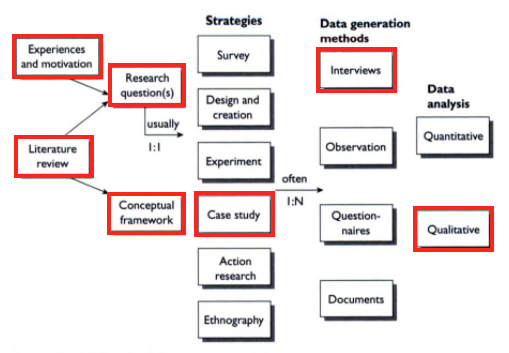
\includegraphics[width=0.75\textwidth]{fig/research_process_master.png}
        \caption{The research process used, marked with methods applied in the research.}
        \label{fig:research_process_master}
    \end{center}
\end{figure}

This project is following a preliminary study, resulting in a project thesis, in the fall of 2019. Starting with a literature review, providing a knowledgeable background as the basis for the project. Moreover, a minor empirical study of the case object, including both interviews and observations. This thesis consists of a more in-depth empirical study, with several interviews as data generators. The conduction of the interviews is with a semi-structured approach, with a set of standardized questions, listed in Appendix \ref{apx:interview_guide}, for every interview. The research process used is shown in figure \ref{fig:research_process_master}.

The interviews for this thesis took place at the project office, near the building site, in Oslo. In line with Norsk Senter for Forskningsdata AS (NSD), the interviews, signing a consent with the participants, were recorded. Moreover, after the interview, the transcript was sent to the participants for them to approve. The interviews lased between 15 minutes and half an hour.

\section{Participants}
The project researcher, Morten Bujordet, is involved in the project, creating the plans, and conducting the research.
	 
Supervising the project is Eric Monteiro. Monteiro is contributing with experience in research in the implementation and use of new digital tools in large scale, as welle as complex organizations. 

Furthermore, Statsbygg, as the manager, has an interest in the project: giving access to the participants in the study. With Darre Brecke Brenden as the point of contact.
	 
In the research, the actors in all layers and disciplines of the project organization will be an aim for the data collection. All personal information gathered will, safely, be stored in a GDPR-compliant Cloud Service, served by NTNU. In the final report, no personal information will be published, and all participants will be anonymized. The participants chosen for the interviews are key personnel leading, modeling, and working in the design of the project. Statsbygg gave a list of 30 candidates, where 16 had the opportunity to participate in the interviews. The interviewees are listed in table \ref{tab:participants}. 

% Please add the following required packages to your document preamble:
% \usepackage{booktabs}
% \usepackage{graphicx}
\begin{table}[]
    \resizebox{\textwidth}{!}{%
    \begin{tabular}{@{}lllll@{}}
    \toprule
    \textbf{Interviewee} & \textbf{Function} & \textbf{Gender} & \textbf{\begin{tabular}[c]{@{}l@{}}Phase 1\\ (November 2019)\end{tabular}} & \textbf{\begin{tabular}[c]{@{}l@{}}Phase 2\\ (February 2020)\end{tabular}} \\ \midrule

        1 & Engineering Manager & Male & & x \\
        2 & BIM Coordinator & Male & & x \\
        3 & Project Manager & Male & & x \\
        4 & Engineering Manager & Male & & x \\
        5 & Engineering Manager & Male & & x \\
        6 & Progress Planner & Female & & x \\
        7 & ITB Manager & Male & & x \\
        8 & Associate & Female & & x \\
        9 & Discipline Leader & Male & & x \\
        10 & Discipline Leader & Female & & x \\
        11 & BIM Manager & Male & & x \\
        12 & Associate & Male & & x \\
        13 & Associate & Male & & x \\
        14 & Discipline Leader & Male & & x \\
        15 & Assiciate & Male & & x \\
        16 & Ass. Project Group Leader & Female & & x \\
        Total interviews & \multicolumn{4}{r}{16} \\ \bottomrule
    \end{tabular}%
    }
    \caption{Overview of interviews and phases of data collection.}
    \label{tab:participants}
\end{table}

\section{Data Analysis}
The analysis started by transcribing the interviews and sent to the participants for approval. Furthermore, utilizing a thematic analysis approach. The thematic analysis followed a set of steps

\begin{enumerate}
    \item A perusal of all the material: It was essential to get to know the material, and to read through all the interviews after the transcription was a vital part of this step. The interviews was ; 
    \item Generation of codes: After getting to know the material it the focus was to identify parts of the text based on the project question, marked with an identifying code; 
    \item Collection of themes: Based on the codes, a set of themes evolved. The codes find most connected were put into groups, based on the connection between them. Which themes adopted in the thesis was based on the research question; 
    \item  Reviewing the themes: Based on the research question, a set of themes was selected. Basing the selection on different criteria, among others, how interesting the theme is, the iteration of the code, and the researcher's considerations; 
    \item Defining and naming the themes: The final collection of themes is selected, and will be the basis for the discussion in the rest of the thesis. The names of the themes are also selected. In this process, three themes appeared, namely: (1) Not unmitigated,(2) Lack of knowledge, and (3) digital potential; 
    \item Producing the report: Describing the findings in the thematic analysis, using the chosen themes as a guideline. Moreover, discussing the themes with relevant literature, previous experience, and context.
\end{enumerate}

The data produced in this process is in the Appendix. The initial codes identified Appendix \ref{apx:codes} and the collection of themes in Appendix \ref{apx:themes}.
Reviewing of themes did not produce much data, due to its subjective manifestation. 

\section{Evaluation of the Method}
The single-case study, as well as the use of unstructured interviews, produce results that cannot be generalized beyond the sample group. Still, they provide a more in-depth understanding of participants’ perceptions, motivations, and emotions. 

One can always argue that utilizing interviews for data collection can tend to be subjective. However, the use of a qualitative approach is best when wanting to describe, contextualize, and gain an in-depth insight into specific concepts or phenomena, which was the case in this empirical study. Furthermore, the project researcher has a part-time job developing the Cogito tool, which can argue for the researcher for being subjective. Though, in this case, 14 of 16 participants mentions Cogito, without the researcher asking them. Also, the participants did not know the relation the researcher had to Cogito; thus, the interviewees spoke freely. Moreover, based on the interviews, the Cogito tool was the one subject getting the most tension; therefore, discussing Cogito and themes related is arguably based on a valid reason. 

The objective of this thesis was to test some of the concluding proposals and observe the change it might bring. Though, due to the COVID-19 virus, the implementation phase was not feasible. Thus, this thesis only consists of a set of proposed actions. Testing of the actions is, therefore, up to a later project, or for the project to do. The project owner has received a summary of this thesis, including the proposed actions. 

Further exploration of the project question is needed to conclude on the matter, moreover, testing of the suggested actions.
\cleardoublepage